\section{Linearen Regression}

Die Idee hinter der Linearen Regression ist, dass zwischen zwei Variablen in einem Datensatz ein Zusammenhang existiert, den man bis auf einen Fehler durch eine lineare Gleichung darstellen kann.

Falls eine solcher Zusammenhang gegeben ist spricht man von einem linearen Modell.
\begin{definition}[Lineares Modell]
    Ein $n$-dimensionaler Zufallsvektor $Y$ genügt einem klassischen linearen Modell, falls es eine Darstellung
    \begin{equation}
        Y=\beta_0 + X^\top \beta+\epsilon
    \end{equation}
    mit Erwartungswert $\Ex[\epsilon]=0$ und Kovarianzmatrix $\Sigma_\epsilon=\sigma^2I_n$.\newline
    Gilt zusätzlich $\epsilon\sim\mathcal{N}(0_n, \sigma^2I_n)$, heißt das Modell \textbf{klassisches lineares Modell}.
\end{definition}
Dabei nennt man den Vektor $Y=[Y_1, \dots, Y_n]^\top\in\R^n$ Regressand oder abhängige Variable und die Matrix $X=[X_1, \dots, X_n]\in\R^{k\times n}$ Regressor oder unabhängige Variable.

Wir betrachten hier nur den Fall des klassischen linearen Modells.

Zur Vereinfachung können wir die Verschiebungskonstante $\beta_0$ und die Steigung $\beta$ zusammenfassen.
Das erlangen wir, indem wir eine $1$ vor den Regressoren $X_i$ anhängen $\tilde{X}_i\coloneqq(1, X_i)\in\R^{k+1}$.

Dadurch erhalten wir 
$$Y= \tilde{X}^\top \tilde{\beta}+\epsilon.$$


Hierbei ist $Y$ gegeben $X$ ein Zufallsvektor, da der Fehler nicht deterministisch ist.

Wenn wir einen Datensatz $\mathcal{D}=\{(X_1,y_1),\dots,(X_n,y_n)\}$ haben, dann betrachten wir Realisierungen von $Y$. Somit ist $y$ deterministisch und wir erhalten den Zusammenhang 
\begin{equation*}
    y_i=\tilde{\beta}^\top \tilde{X_i}+\epsilon_i  \quad\mathrm{bzw.}\quad y=\tilde{X}^\top\tilde{\beta}+\epsilon.
\end{equation*}
Das Ziel der linearen Regression ist es für eine gegebene Realisierung $y$ von $Y$ den Vektor $\tilde{\beta}$ schätzen.

Der gleichmäßig beste erwartungstreue Schätzer (UMVU) der linearen Regression ist durch den Kleinste-Quadrate-Schätzer gegeben.

\subsection{Kleinste-Quadrate-Schätzer}

Der KQ-Schätzer minimiert den quadratischen Abstand der Realisierungen $y_i$ und der Schätzungen $\hat{y}_i=\hat{\beta}^\top\tilde{X}_i$, in Formeln
\begin{equation}
    \hat{\beta} = \argmin_{\tilde{\beta}\in\R^{k+1}}\sum_{i=1}^n\left|y_i-\tilde{\beta}^\top\tilde{X}_i\right|^2.
\end{equation}

Diesen Minimierer kann explizit angegeben werden.
\begin{satz}[KQ-Schätzer in linearen Modellen]\label{stz:kqs}
    Sei $Y = X + \epsilon$ ein lineares Modell
    mit einer $(k + 1)\times n$-Matrix X und $rg(X) = k + 1$, dann ist für eine beobachtete Realisierung
    $y$ von $Y$ der KQ-Schätzer $\hat{\beta}$ gegeben durch
    \begin{equation}
        \hat{\beta}=(\tilde{X}\tilde{X}^\top)^{-1}\tilde{X}y.
    \end{equation}
    $\hat{\beta}$ ist ein erwartungstreuer Schätzer für $\beta$ mit Kovarianzmatrix $\Sigma_{\hat{\beta}} = \sigma^2(\tilde{X}\tilde{X}^\top)^{-1}$.
\end{satz}
\begin{proof}
    Übungsaufgabe.
\end{proof}

Nach dem verallgemeinerten Gauß-Markov-Theorem, siehe \cite[][Satz 5.5.14]{ruschendorf2014mathematische}, ist dieser Schätzer insbesondere der gleichmäßig beste Schätzer.

Die Darstellung des KQ-Schätzers aus Satz \ref{stz:kqs} haben wir verwendet, um unsere Schätzfunktion zu implementieren, siehe Auszug aus dem Code \ref{lst:umvubeta}.

\noindent\begin{minipage}{\linewidth}
\lstinputlisting[language=Python, caption=Simple lineare Regression aus der Datei \lstinline{regression.py}, firstline=34, lastline=44, firstnumber=34, label=lst:umvubeta]{../code/regression.py}
\end{minipage}

Wir wollen die Abhängigkeit der Gesamtrechnung und dem gegebenem Trinkgeld berechnen. Dabei betrachten wir die Gesamtrechnung als Regressor mit einer Dimension ($k=1$) und das Trinkgeld als Regressand.
Durch \lstinline|statsmodels.api.OLS| können wir uns verschiedene statistische Werte des KQ-Schätzer ausgeben lassen, siehe \cref*{tab:regression}.

\begin{table}[]
    \begin{center}
\begin{tabular}{lclc}
\toprule
\textbf{Dep. Variable:}    &       tip        & \textbf{  R-squared:         } &     0.457   \\
\textbf{Model:}            &       OLS        & \textbf{  Adj. R-squared:    } &     0.454   \\
\textbf{Method:}           &  Least Squares   & \textbf{  F-statistic:       } &     203.4   \\
\textbf{Date:}             & Wed, 30 Aug 2023 & \textbf{  Prob (F-statistic):} &  6.69e-34   \\
\textbf{Time:}             &     15:50:13     & \textbf{  Log-Likelihood:    } &   -350.54   \\
\textbf{No. Observations:} &         244      & \textbf{  AIC:               } &     705.1   \\
\textbf{Df Residuals:}     &         242      & \textbf{  BIC:               } &     712.1   \\
\textbf{Df Model:}         &           1      & \textbf{                     } &             \\
\textbf{Covariance Type:}  &    nonrobust     & \textbf{                     } &             \\
\bottomrule
\end{tabular}
\begin{tabular}{lcccccc}
               & \textbf{coef} & \textbf{std err} & \textbf{t} & \textbf{P$> |$t$|$} & \textbf{[0.025} & \textbf{0.975]}  \\
\midrule
\textbf{const} &       0.9203  &        0.160     &     5.761  &         0.000        &        0.606    &        1.235     \\
\textbf{x1}    &       0.1050  &        0.007     &    14.260  &         0.000        &        0.091    &        0.120     \\
\bottomrule
\end{tabular}
\begin{tabular}{lclc}
\textbf{Omnibus:}       & 20.185 & \textbf{  Durbin-Watson:     } &    2.151  \\
\textbf{Prob(Omnibus):} &  0.000 & \textbf{  Jarque-Bera (JB):  } &   37.750  \\
\textbf{Skew:}          &  0.443 & \textbf{  Prob(JB):          } & 6.35e-09  \\
\textbf{Kurtosis:}      &  4.711 & \textbf{  Cond. No.          } &     53.0  \\
\bottomrule
\end{tabular}
%\caption{OLS Regression Results}
\end{center}

Notes: \newline
 [1] Standard Errors assume that the covariance matrix of the errors is correctly specified.
    \caption[bla]{Zusammenfassung der OLS Regressions Statistik.}
    \label{tab:regression}
\end{table}

Dadurch könnte hier eine ausführliche Analyse dieser statistischen Werte stehen. 

Über unsere eigens implementierten Funktionen haben wir die Daten in einem Scatterplot dargestellt und die Regressionsgerade einzeichnen, siehe \cref*{fig:regression}

\begin{figure}
    \centering
    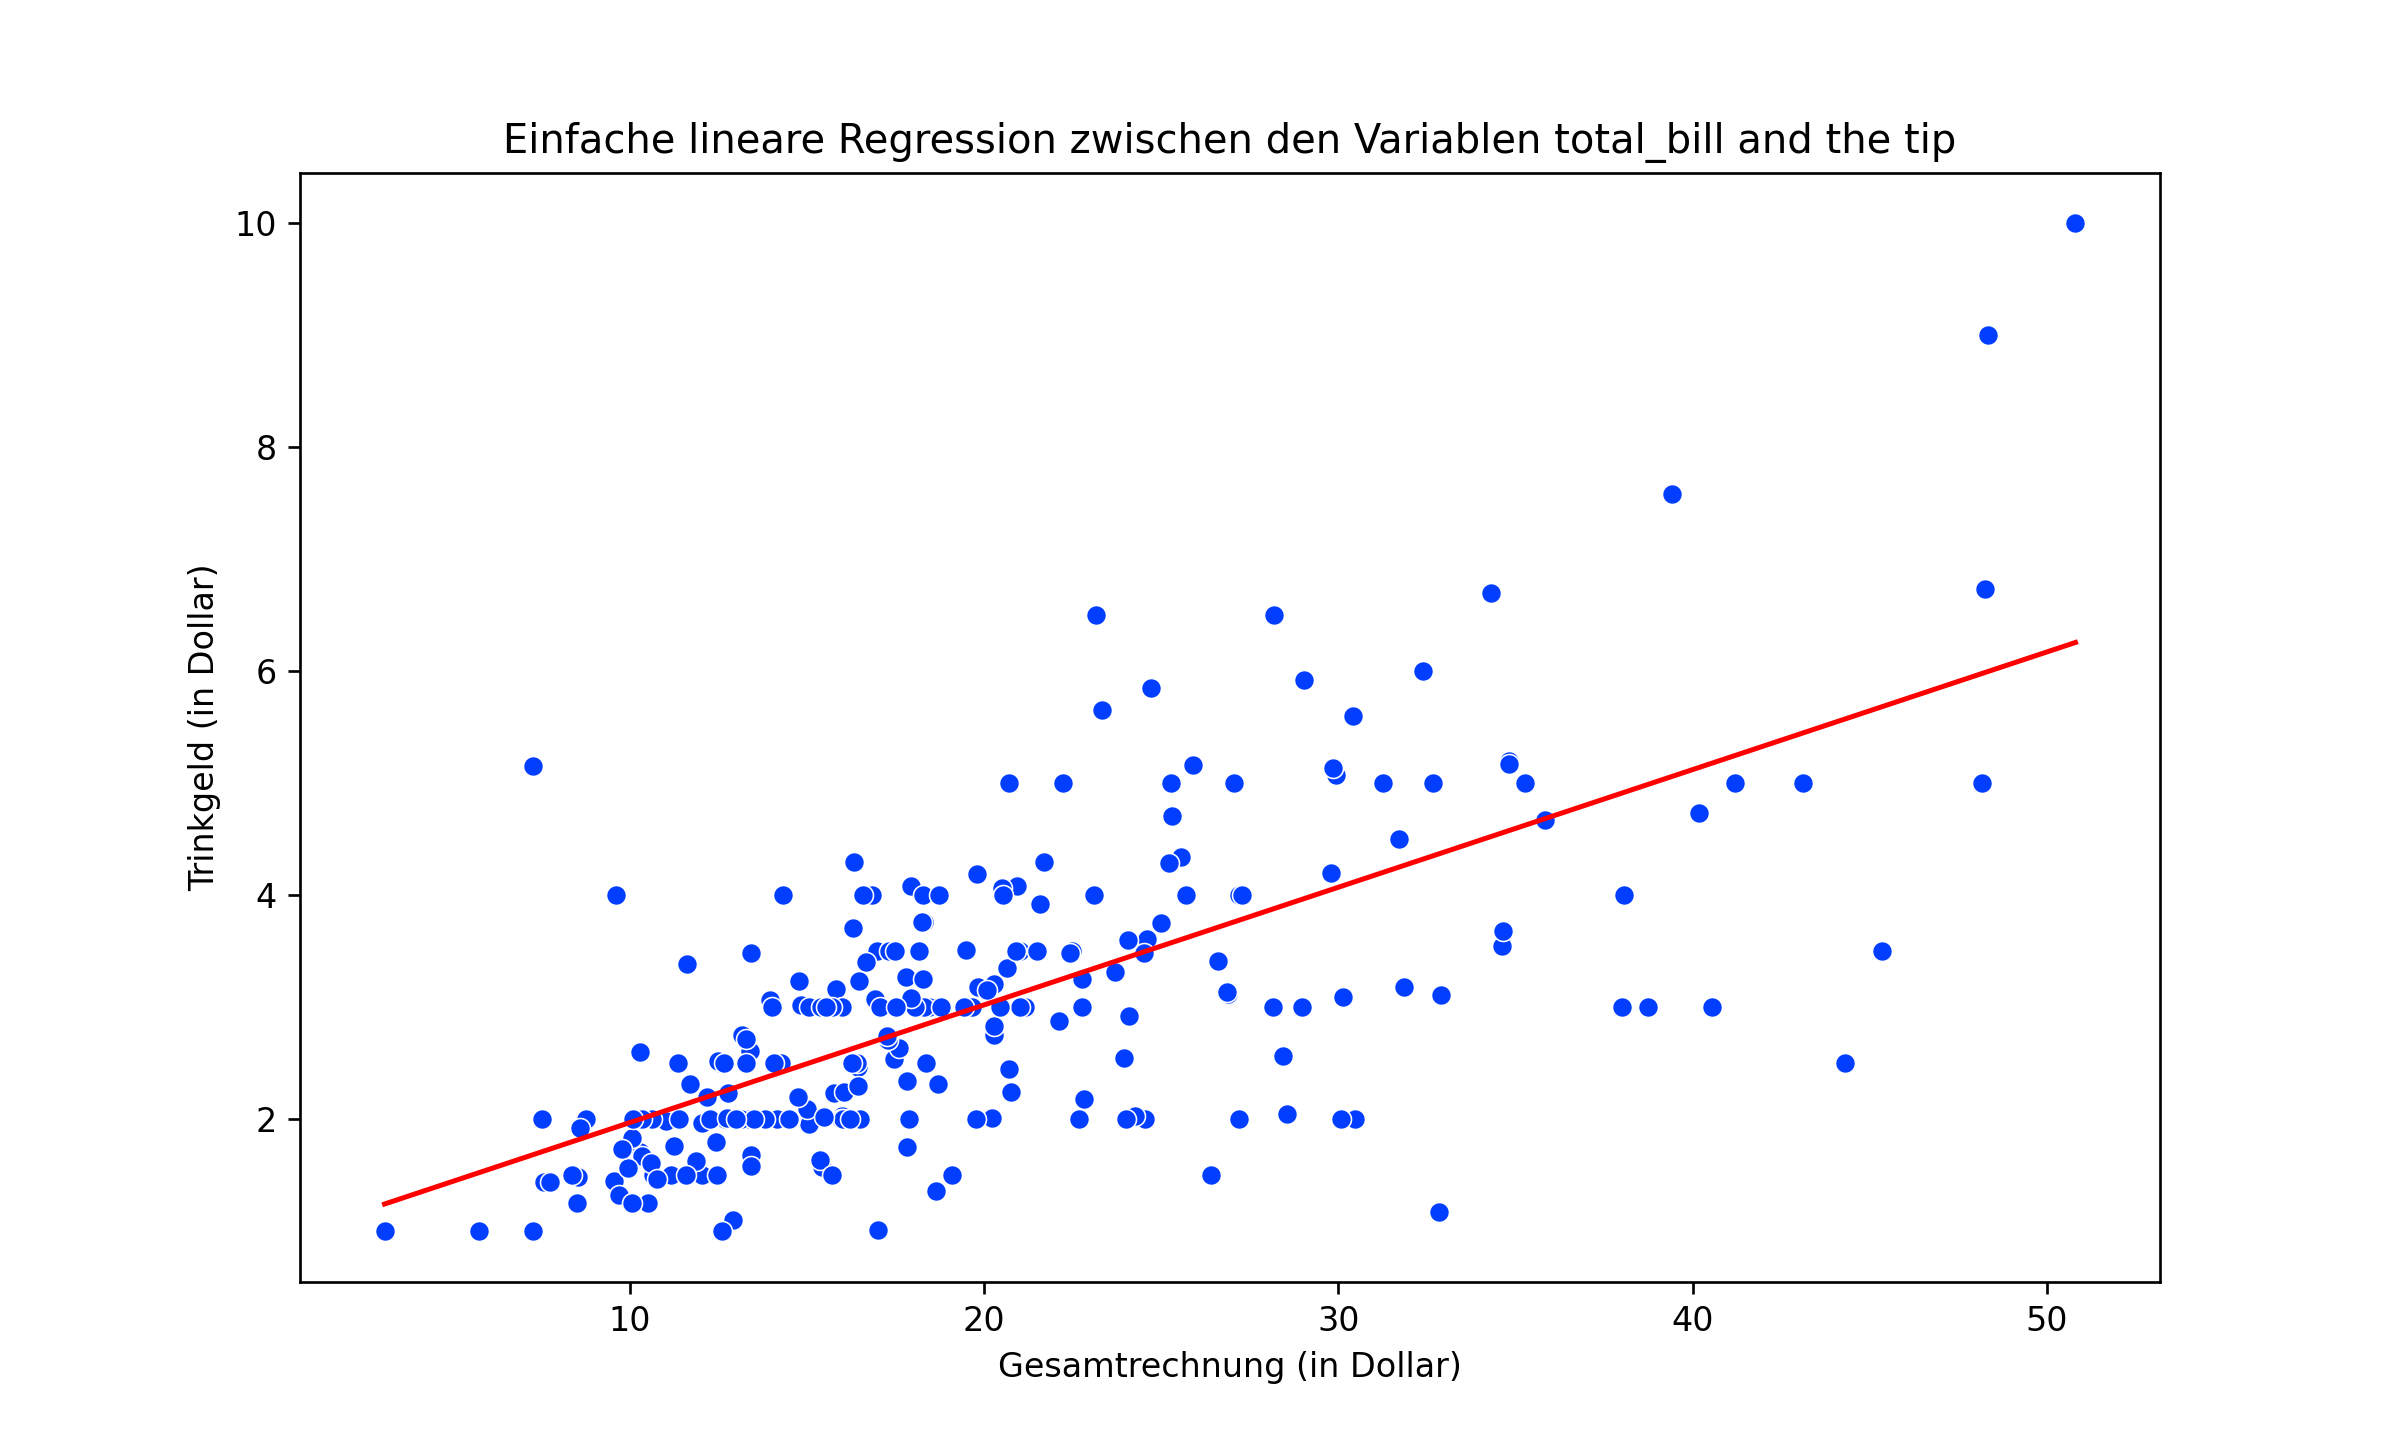
\includegraphics[scale=0.17]{../figures/simple_reg.png}
    \caption{In einen Scatterplot eingezeichnete selbstimplementierte Regressionsgerade.}
    \label{fig:regression}
\end{figure}

\subsection{p-Wert}

\dots

\subsection{Konfidenzband für eine Lineare Regression}

\dots
